\subsection{Configuração do Cliente Outlook 2003}

Para configurar a conta de email no Outlook 2003\footnote{A configuração de versões anteriores do Outlook (2000 e XP) é análoga.} deverá ir ao menu tools e seguidamente escolher a opção ``Email Accounts'' tal como na seguinte imagem.

\begin{figure}[H]
    \begin{center}
        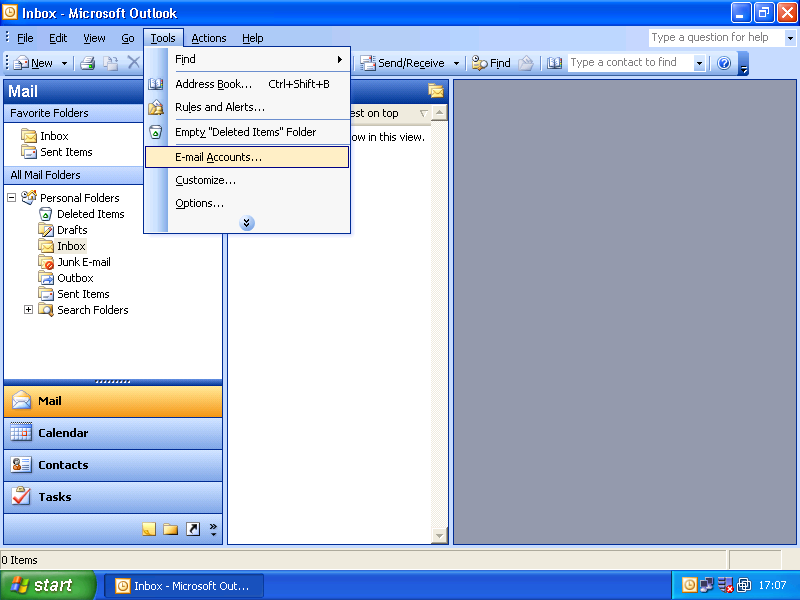
\includegraphics[width=10cm]{include/img/outlook2003_1}
    \end{center}
    \caption{Ecrã inicial Outlook 2003}
    \label{fig:OUTLK2k31}
\end{figure}

De seguida deverá escolher na opção "Add a new e-mail account" e carregar no botão "Next" como a imagem seguinte:

\begin{figure}[H]
    \begin{center}
        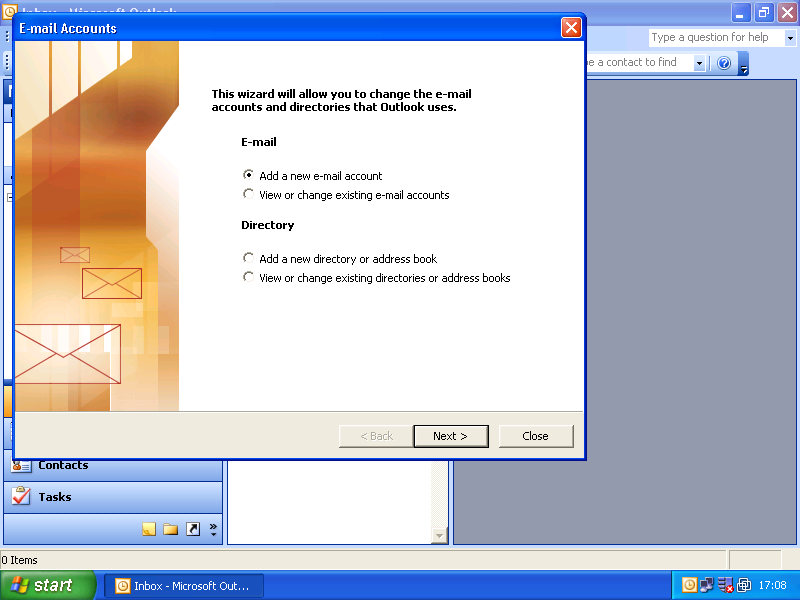
\includegraphics[width=10cm]{include/img/outlook2003_2}
    \end{center}
    \caption{Criação de conta de email - 1}
    \label{fig:OUTLK2k32}
\end{figure}

Deverá escolher POP3 ou IMAP e carregar em "Next".

\begin{figure}[H]
    \begin{center}
        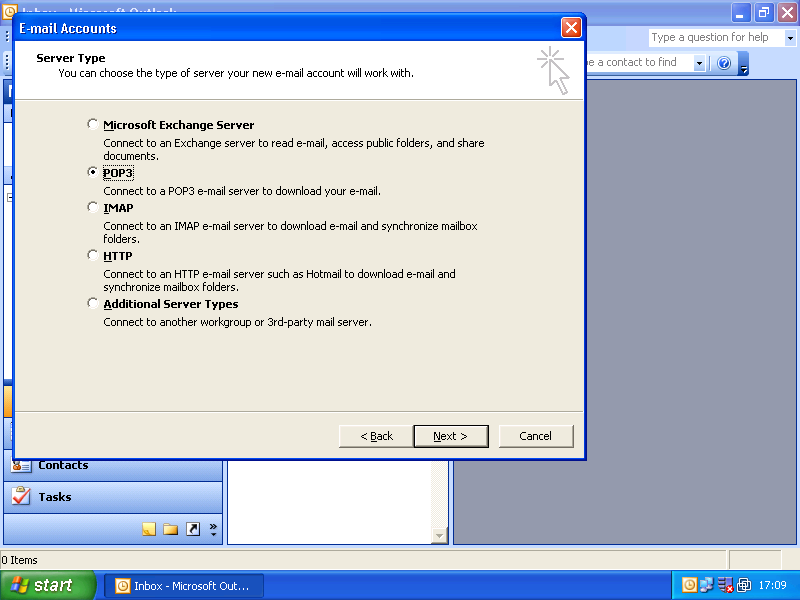
\includegraphics[width=10cm]{include/img/outlook2003_3}
    \end{center}
    \caption{Criação de conta de email - 2}
    \label{fig:OUTLK2k34}
\end{figure}

Inserir na caixa "Your Name" o seu nome, na caixa "E-mail Address" o endereço de email que será algo como utilizador@dominio.pt. Poderá variar consoante o seu endereço de correio.

Na caixa "Incoming mail server" deverá inserir o endereço do seu servidor de email, algo como "mail.dominio.pt". Este endereço poderá variar.

Na caixa "Outgoing mail server" deverá inserir o servidor de correio para enviar. Caso não seja indicado nada em contrário deverá inserir o mesmo que escreveu no "Incoming mail server".

Na caixa "User Name" deverá inserir o seu endereço de email novamente enquanto que na caixa "Password" deverá inserir a sua palavra-passe. Poderá escolher a opção "Remember password". De seguida deverá carregar no botão "More settings".

\begin{figure}[H]
    \begin{center}
        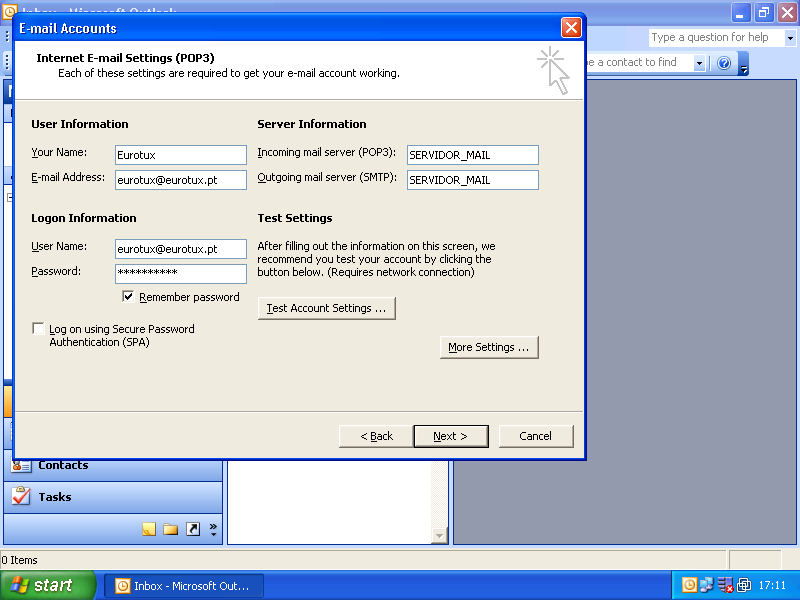
\includegraphics[width=10cm]{include/img/outlook2003_4}
    \end{center}
    \caption{Criação de conta de email - 3}
    \label{fig:OUTLK2k35}
\end{figure}

Na caixa "Internet E-mail Settings" deverá escolher a secção "Outgoing server" e escolher a opção "My outgoing server (SMTP) requires autentication" e a opção "Use same settings as my incoming mail server". De seguida deverá entrar na secção "Advanced".

\begin{figure}[H]
    \begin{center}
        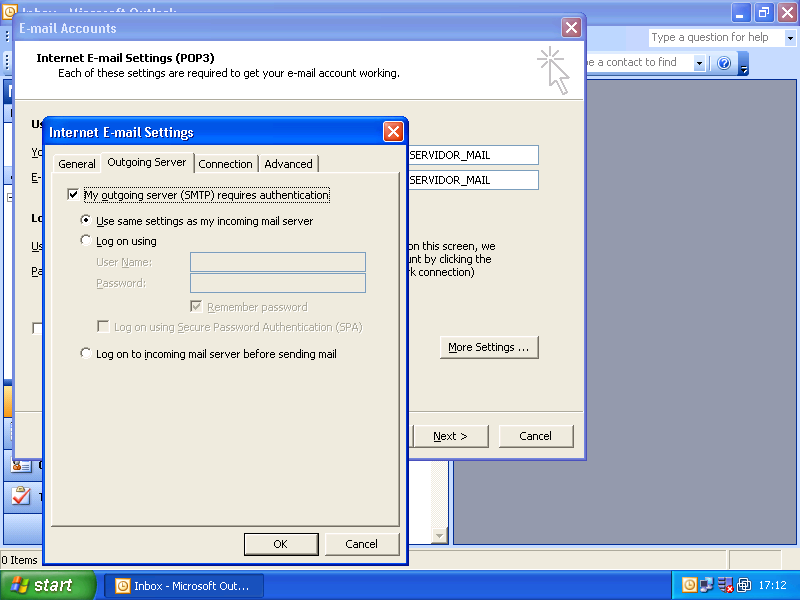
\includegraphics[width=10cm]{include/img/outlook2003_5}
    \end{center}
    \caption{Criação de conta de email - 4}
    \label{fig:OUTLK2k36}
\end{figure}

Na secção "Advanced" no incoming server deverá escolher a opção "This server requires and encrypted connection (SSL)". Note que a porta automaticamente irá mudar para 995 (no caso de ter escolhido anteriormente o POP3) ou 993 (no caso de ter escolhido anteriormente IMAP). Deverá de seguida carregar no botão "OK".

\begin{figure}[H]
    \begin{center}
        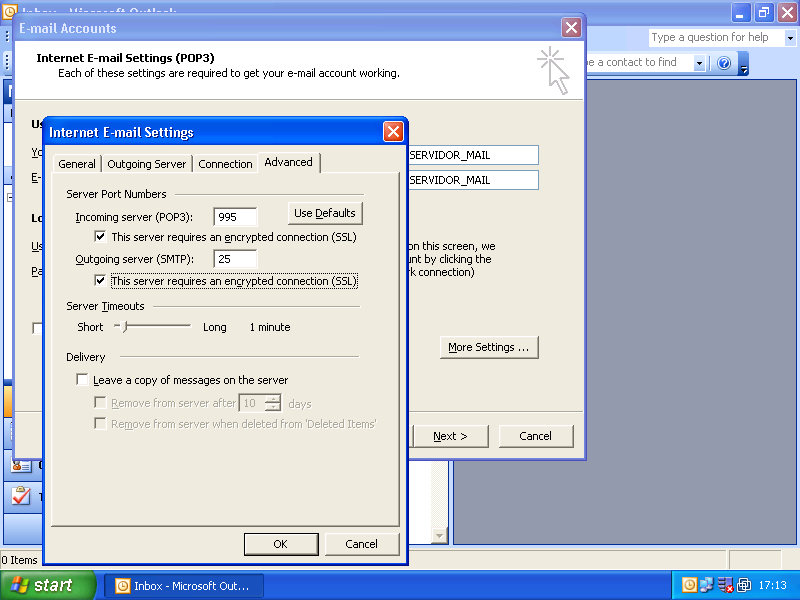
\includegraphics[width=10cm]{include/img/outlook2003_6}
    \end{center}
    \caption{Criação de conta de email - 5}
    \label{fig:OUTLK2k37}
\end{figure}

Deverá carregar agora no botão "Finish" para terminar a criação da conta de correio.
Ser-lhe-á apresentado um ecrã similar ao seguinte com a conta de correio criada. Deverá carregar em "Close" para fechar a gestão das contas de correio.

\begin{figure}[H]
    \begin{center}
        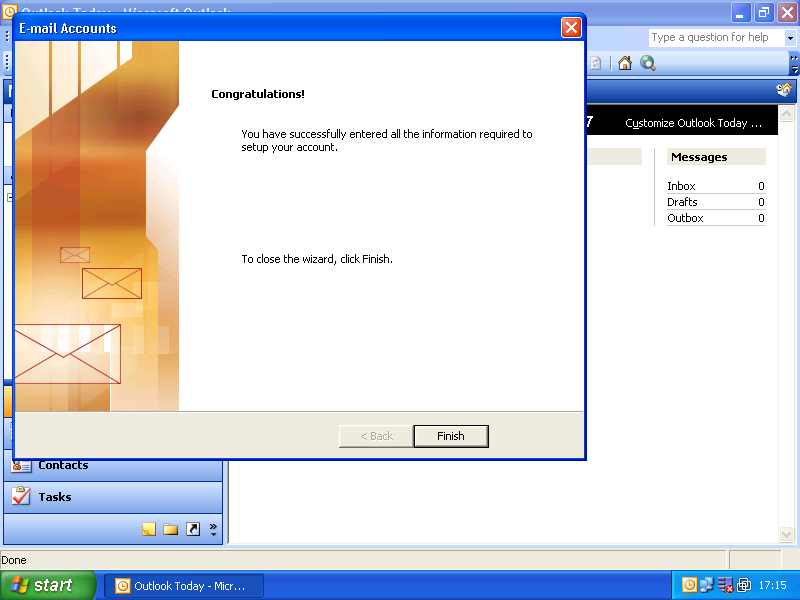
\includegraphics[width=10cm]{include/img/outlook2003_7}
    \end{center}
    \caption{Criação de conta de email - 7}
    \label{fig:OUTLK2k39}
\end{figure}

